%%%%%%%%%%%%%%%%%%%%%%%%%%%%%%%%%%%%%%%%%
% Journal Article
% LaTeX Template
% Version 1.3 (9/9/13)
%
% This template has been downloaded from:
% http://www.LaTeXTemplates.com
%
% Original author:1
% Frits Wenneker (http://www.howtotex.com)
%
% License:
% CC BY-NC-SA 3.0 (http://creativecommons.org/licenses/by-nc-sa/3.0/)
%
%%%%%%%%%%%%%%%%%%%%%%%%%%%%%%%%%%%%%%%%%

%----------------------------------------------------------------------------------------
%	PACKAGES AND OTHER DOCUMENT CONFIGURATIONS
%----------------------------------------------------------------------------------------

\documentclass{llncs}
\usepackage[utf8]{inputenc}
\usepackage[T1]{fontenc}
\usepackage{lmodern}
\usepackage{subfig}

\usepackage{hyperref} % For hyperlinks in the PDF
\usepackage{graphicx}

%----------------------------------------------------------------------------------------
%	TITLE SECTION
%----------------------------------------------------------------------------------------

\title{A Cross-Platform Assessment of Energy Consumption in Evolutionary Algorithms}
\subtitle{Towards Energy-Aware Bioinspired Algorithms}

\author{F. Fernández de Vega \inst{1} \and F. Ch\'avez\inst{1} \and J. D\'iaz\inst{1} \and J.A. Garc\'ia\inst{1} \and P.A. Castillo\inst{2} \and Juan J. Merelo\inst{2} \and C. Cotta\inst{3}\\
\institute{ Universidad de Extremadura \\
{\email{\{fcofdez,fchavez,mjdiaz,jangelgm\}@unex.es}} \\
\and ETSI Inform\'atica, Universidad de Granada\\
{\email{\{pacv,jmerelo\}@ugr.es}} \\ 
\and ETSI Inform\'atica, Campus de Teatinos, Universidad de M\'alaga\\
{\email{ccottap@lcc.uma.es}} \\
}}

%----------------------------------------------------------------------------------------

\begin{document}

\maketitle % Insert title

%----------------------------------------------------------------------------------------
%	ABSTRACT
%----------------------------------------------------------------------------------------

\begin{abstract}
Energy consumption is a matter of paramount importance in nowadays 
environmentally conscious society. It is also bound to be a crucial issue
in light of the emergent computational environments arising from the 
pervasive use of networked handheld devices and wearables. Evolutionary
algorithms (EAs) are ideally suited for this kind of environments due to their
intrinsic flexibility and adaptiveness, provided they operate on viable
energy terms. 
%In this work we analyze the energy requirements of different EAs 
In this work we analyze the energy requirements of a genetic programming (GP) algorithm 
on several computational platforms and study the impact that 
parameterization has on these requirements, paving the way for a future
generation of energy-aware EAs.  As experimentally demonstrated, handheld devices and tiny computer models mainly use for educational purposes may be the most energy efficient ones when looking for solutions by means of GP.
\end{abstract}

\noindent \textbf{Keywords:} Green computing, energy-aware computing,
performance measurements, evolutionary algorithms. 

%----------------------------------------------------------------------------------------
%	ARTICLE CONTENTS
%----------------------------------------------------------------------------------------

\section{Introduction}

The analysis of evolutionary algorithms typically relies on computational complexity \cite{complexity}, %this is not an and. Change it - JJ
 and even when sometimes it is not possible to diminish it, processor
 companies try to offer new products providing higher performance.
 Thus, \textit{multi-core and many-core} processors allow to run
 parallel applications on desktop computers, but indirectly imply the
 need of learning new parallel programing paradigms and libraries. % don't see anything coming here - JJ  

Despite the advantages provided by these models, an important feature
is frequently forgotten:  power consumption, which largely correlates
with performances provided by new processors. That is why, in an
environment where raw processor speed is no longer doubling at an
accelerated pace, reducing power consumption and taking it into
account when evaluating algorithms becomes an issue, to the point that
latest HPC benchmarks also include this measurement in their reports
and there are calls for {\em energy-proportional computing}
\cite{barroso2007case} and 
% Thus, although new
% hardware capabilities allows to significantly reduce computing time,
% the cost of electricity required to run the algorithms is not always
% taken into account.% it is definitely not. When speed is not
                   % increasing, and it is not, the most important
                   % feature is consumption. You could talk about
                   % Moore's law here (or its end thereof) - JJ
                   
                   % Feel free to talk yourself, JJ.  - Paco.
% Done :-) - JJ
\textit{green computing} \cite{green-computing}, a term that was born in the last decade to refer
to problems associated to power consumption in computing environments,
particularly in large data centers. But this
energy-aware and proportional point of view is equally applicable to desktop computers
and any kind of algorithms that may be run. 

When dealing with evolutionary algorithms (EAs), big efforts have been
applied to improve performances while applying parallel and
distributed systems \cite{paba}.  Improvements have tried to analyse
global quality of solutions when compared with time required to find
them.   
But similarly as the traveller considering not only speed but also
price when selecting means of transport, we should also consider
energy consumption when running an algorithm, and not just the time to
solution.  % this sentence (or similar) should be included in the
           % abstract  -  pedro 

To the best of our knowledge, the influence of this important
parameter has not been analysed yet in the context of EAs, although
its importance has already been recognised \cite{ephemeral}.  This is
the main goal of this work, to make a preliminary analysis of the
impact of power consumption when running EAs on different hardawre
architectures, so that we may in the future be aware of the
importance, and even design energy-aware EAs. 

The rest of the paper is organized as follows:  Section \ref{eas}
describe previous works on the area;  section \ref{methodology}
describes the experiments performed and section \ref{results} shows
the results obtained.  Finally we summarize our conclusions in section
\ref{conclusions}. 

% I think we should include here the description of the paper structure, i.e., the "The rest of the paper is structured as follows:"
%  - pedro



\section{Evolutionary Algorithms and Energy Consumption}
\label{eas}

Computer science took interest in energy efficiency a number of years
ago, and a new research topic was born, \textit{Green Computing}
\cite{hooper2008}, together with the \textit{energy-aware}
\cite{barroso2007,energy-aware} concept. Even processor 
makers offered new processors providing \textit{dynamic frequency
  scaling}, which adapts energy consumption as well as heat dissipation
to the need of the processes to be run \cite{Bansal2004,albers2011,energy-efficient}. 


On the other hand, EAs have already been applied as optimization
algorithms in the context of energy management.  We can thus find
optimization problems associated to HVAC (Energy management of
heating, ventilating and air-conditioning) \cite{Fong2006},
\cite{Lee2011}.  We can also find EAs applied to energy dispatch
\cite{Fadaee2012}.  But any of the above referred problems are only
tangentially connected to the problem we are interested in:  how to
include energy consumption as one of the main features of EAs to be
considered when looking for solutions, and its relationship with the
main parameters of the algorithm. 

The main concept discussed in this paper is the capability of an EA to adapt
to dynamic environments in which energy consumption is one of the main
components to be optimized \cite{ephemeral2015}. This capability, which
is one of the self-$\star$ features of a
given algorithm, including EAs \cite{ephemeral2015}, has already been
considered by researchers in other kind of algorithms and computer architectures \cite{Almeida2013}, in some cases
an essential part of them \cite{energy-aware}. Energy-awareness is
considered a key
component in infrastructures of any size, from large data centers to
processor architectures for mobile devices where battery life must be
optimized.  Also in this context, EAs have been employed to design
cache hierarchies reducing energy consumption and heat dissipation
\cite{DiazAlvarez2016}. 

Yet, to the best of our knowledge, EAs have never been studied from
the point of view of their own energy needs. 
Given their stochastic nature, the number of parameters regulating the
way they perform the search process and the plethora of hardware
platforms available to run them, we consider it of interest to study
the energy consumed when looking for a solution, so that in the future
they may become energy-aware and capable of self-regulating when
progressing towards the solution of the problem faced. This is what we
have set out to do in this paper.

%This is part of our first approach to the study of EAs energy
%consumption.  Although we have already performed a preliminary study
%with EAs \cite{MAEB}, we try here to analyze a widespread software
%tool devoted to GP, \textit{lilgp}, so that we can reach wider
%conclusions. 

%I think that this paragraph can't be included, because the MEAB 2016 is later than PPSN. - Paco Chávez

% maybe this paragraph should be at the end of the introduction section instead of at the end of literature section  -  pedro
%The rest of the paper is organized as follows:  
% It's there already

\section{Methodology}
\label{methodology}

This preliminary study tries to measure power consumption for a couple
of EAs, Genetic Algorithms (GA) and Genetic Programming (GP). 

\subsection{Algorithmic Setting}

Given the stochastic nature of this kind of algorithms, we firstly decided to run each of the experiment 30 times so that the average can be computed as an estimation of the algorithm behavior.  On the other hand, and given that different hardware platforms will be tested, we decided to choose 30 random seeds so that all of the runs are exactly the same in every platform, when considering high level operations defined in the high level programming language.

On the other hand, and given the influence of computing time in the total amount of energy consumed by the algorithm, we configured the main loop of the algorithm to finish when a required level of solution quality is reached. We are thus mainly interested in the average computing time for the 30 runs, together with the energy consumed along that time.  The only differences that may arise are due to hardware differences:  instruction set architecture, processor speed, operating system, etc;  % also the operating system architecture affects  -  pedro
features that are not in the focus of this work.  Nevertheless, theses differences may influence future decision on the preferred hardware for the algorithms.  

We must also mention the interest in studying some of the main parameters of the algorithm:  they have a well-known impact on the time to find solutions, and may thus also directly, or indirectly influence the energy consumed to reach that solution.  In this preliminary study we have focused on population size and have tested several values for each of the algorithms tested.

In order to ease the compilation processes in every hardware platform, we have selected on the one hand a simple GA \cite{michalewicz} with a simple C-implementation \cite{web_algoritmo}, and on the other hand lilgp for GP \cite{lilgp}.  

Regarding the problems selected for the experimental stage, we have selected one of the test problems provided with each of the software tools selected:  the multiplexer problem provided with lilgp on the one hand, and an scalar function -check ~\ref{eq:fitness}-  with five variables to be optimized. 

Main parameters for both the GA and the GP problems are described in Table~\ref{Table:par_ga} and Table~\ref{Table:par_gp}.  The upper limit for generation number is  $10000$, stopping the run when the best individuals is ($0,999\%$) near the optimal solution. Four population sizes have been tested.

\begin{table}
%\renewcommand{\arraystretch}{1.3}
\centering
\caption{Main GP Parameters for multiplexer 6.}
\label{Table:par_gp}
\begin{tabular}{cc}
\hline
%Max number of generation & $10000$ \\
Max number of generations & $500$ \\
%Population sizes & $50$,$100$,$500$,$1000$ \\
Population sizes & $100$,$200$,$400$,$500$,$1000$ \\
Crossover probability & $0.8$ \\ 
Mutation probability & $0.15$ \\ 
%Other parameters &  default values for the problem in \cite{lilgp} \\
\hline
\end{tabular}
\end{table}


\subsection{Computational Platforms}

Table~\ref{Table:devices} provide detals for hardware architectures tested. 
\begin{table}
%\renewcommand{\arraystretch}{1.3}
\centering
\caption{Devices}
\label{Table:devices}
\begin{tabular}{ccccc} \hline
Device		&	Processor			&	Cores	&	RAM \\ \hline
Raspberry Pi	& Cortex-A7 (900 Mhz)	& 4 			&	1GB \\
Tablet		& Samsung Galaxy Tab-3 (SM-T311) (1,5 GHz)& 2  & 1.5 GB \\
Laptop 		& Intel(R) Core(TM) i5-2450M (2.5GHz)	&	4	&	8GB\\
iMac			& Intel(R) Core(TM) i5  (2.7GHz)	& 4	& 4GB \\
Blade		& Virtual Machine (on IBM 8CPUs x 2GHz, \\
&Intel Xeon CPUE5504 @ 2.00GHz (x2), 16Gb RAM)) & 4 & 4GB \\
% this table should be updated with the information about the Android tablet:
%   SAMSUNG GALAXY TAB-3 (SM-T311)
%   Android 4.4.2
%   Kernel 3.0.31
%   CPU 1.5 GHz dual core
%   Samsung Exynos 4212 Dual SoC processor
%   1.5GB RAM
\hline
\end{tabular}
\end{table}

Given differences among hardware devices, we have employed different means  % means???  
for measuring energy consumed by each of the algorithms.  
\subsubsection*{Laptop and Raspberry Pi.}
Regarding the desktop PC and raspberry pi, we have employed a voltimeter for measuring total consumption of the device in two different scenarios:  (i) when the algorithm is not running and (ii) when the algorithm is running.  Given that \textit{current intensity} values remain constant in every case, we can obtain the measure for the algorithm by simply substracting both values for a given device.  This value together with electric tension allows us to compute watts consumed.

\subsubsection*{Tablet.}
When android devices are considered, such as smartphones or tablets, we have employed  \textit{PowerTutor} \cite{powertutor},\cite{powertutor2}. This app allows to check energy consumption for every process run.

With that information, we can compute kilowats-hour (kwh).  This will be our main measure to compare the behavior of the algorithm in every hardware platform.

\subsubsection*{iMac.}
Data collection in the iMac was done using \emph{HardwareMonitor}\footnote{\url{http://www.bresink.com/osx/HardwareMonitor.html}}. 
This application suite includes a command-line tool that provides readings of the internal
hardware sensors built on the computer. In order to obtain power measurements, a shell
script is run in parallel to each run of the EA. This script gathers sensor data periodically
(we use a sampling frequency of 1s) and goes to sleep state between measurements. 
During the experimentation, no other application is run, apart from background processes 
under OS control. 
To gauge the data,
the same data-collection process is run for 100s before each batch of runs, thus providing
an indication of the system basal consumption at that moment which is in turn used to 
compute the excess power consumption due to the EA (and hence accounting for
eventual hysteretic phenomena).

\subsubsection*{Blade.}

\subsubsection*{FPGA.}


%Para realizar la experimentación, y tal como se describe en la sección previa, en primer lugar  hemos seleccionado el conjunto de dispositivos descritos en la Tabla~\ref{Table:devices}. 


When the Xilinx FPGA has been tested using the evaluation kit described in Table~\ref{Table:devices} to compile the GA algorithm. Given the way the algorithms are converted into hardware components, the stop criteria cannot be applied, and instead, the average number of generations computed in other hardware platforms has been employed as the upper limit for the run, given that the same random seeds will produce the same high level operations for the algorithm.  The total ammount of generation for population sizes of 50, 100, 500 and 1000 individulas are  6505, 5859, 2732 y 1684, respectively.


%Las características particulares del entorno donde se implementa el algoritmo se especifican en la Tabla~\ref{Table:devices}.

\begin{table}
\renewcommand{\arraystretch}{1.3}
\centering
\caption{FPGA hardware}
\label{Table:fpga}
\begin{tabular}{cc} \hline
  Version & Vivado v.2015.4 (win64) Build 1412921 Wed Nov 18 09:43:45 MST 2015 \\ 
  Device & xc7z020clg484-1\\
\hline
\end{tabular}
\end{table}

When the FPGA SoC ZC702 has been employed, together with the IP module required for the algorithm, a proprietary Xilnx IP module was required to launch and connect the algorithm with input/output.  This means that a number of extra hardware resources are required (LUT, LUTRAM, FF, BRAM, DSP, BUFG) which will increase power consumption.  

%\begin{table}
%\renewcommand{\arraystretch}{1.3}
%\centering
%\caption{Característica de los dispositivos.}
%\label{Table:devices}
%\begin{tabular}{cccc} \hline
%Dispositivo&Procesador&Núcleos&RAM\\ \hline
%Raspberry Pi& Cortex-A7 (900 Mhz)& 4 &1GB \\
%Laptop & Intel(R) Core(TM) i5-2450M (2.50GHz)&4&8GB\\
%Xilinx ZYNQ-7000 SoC ZC702 (50Mhz) & & \\
%\hline
%\end{tabular}
%\end{table}

\begin{equation}
\label{eq:fitness}
 F=x_{1}^{4} + (x_{2}^{3} * x_{3}^{2}) - (x_{3} * x_{4}) + x_{5} 
\end{equation}




\begin{table}
\renewcommand{\arraystretch}{1.3}
\centering
\tiny
\caption{Main GA parameters.}
\label{Table:par_ga}
\begin{tabular}{cc}
\hline
Max number of generations & $10000$ \\
Population sizes & $50$,$100$,$500$,$1000$ \\
Crossover probability & $0.8$ \\ 
Mutation probability & $0.15$ \\ 
\hline
\end{tabular}
\end{table} 


\section{Results}
\label{results}



\begin{table}[!t]
\caption{Time (in seconds) for lilgp-multiplexer-6 run on each system depending on the population size. The numbers denote the mean and the standard error of the mean for the 30 runs performed.}
\label{T:r_obtained}
\begin{tabular}{lrcrcrcrcrc}
&&\multicolumn{9}{c}{population size}\\
\cline{3-11}
System 		&~~& 100	&~& 200	&~& 400	&~& 500	&~& 1000\\
\hline
\raspberry	&& 7.77 $\pm$ 1.31	&& 19.91 $\pm$ 2.41	&& 46.22 $\pm$ 4.01	&& 61.10 $\pm$ 7.19	&& 116.80 $\pm$ 13.55	\\
\laptop	&& 1.73 $\pm$ 0.31	&& 4.43 $\pm$ 0.54	&& 10.60 $\pm$ 0.97	&& 13.89 $\pm$ 1.68	&& 27.13 $\pm$ 3.36	\\
\iMac	&& 1.38 $\pm$ 0.28	&& 3.69 $\pm$ 0.48	&& 8.98 $\pm$ 0.84	&& 11.74 $\pm$ 1.44	&& 22.95 $\pm$ 2.85	\\
\tablet	&& 4.43 $\pm$ 0.75	&& 4.85 $\pm$ 0.78	&& 35.68 $\pm$ 4.15	&& 36.17 $\pm$ 4.17	&& 68.70 $\pm$ 7.89	\\
\blade	&& 2.59 $\pm$ 0.53	&& 6.88 $\pm$ 0.91	&& 16.78 $\pm$ 1.59	&& 22.28 $\pm$ 2.77	&& 43.53 $\pm$ 5.48	\\
\hline
\end{tabular}
\end{table}

\begin{figure}[!t]
\subfloat[\label{fig:power}]{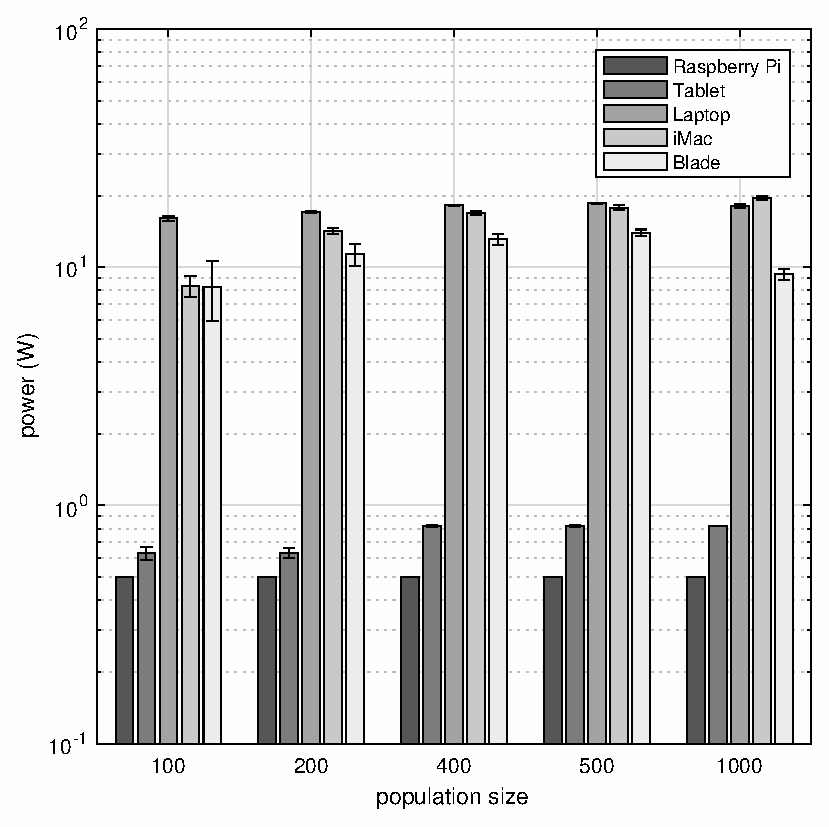
\includegraphics[width=.48\textwidth]{excess_power_log_2.eps}}~~
\subfloat[\label{fig:energy}]{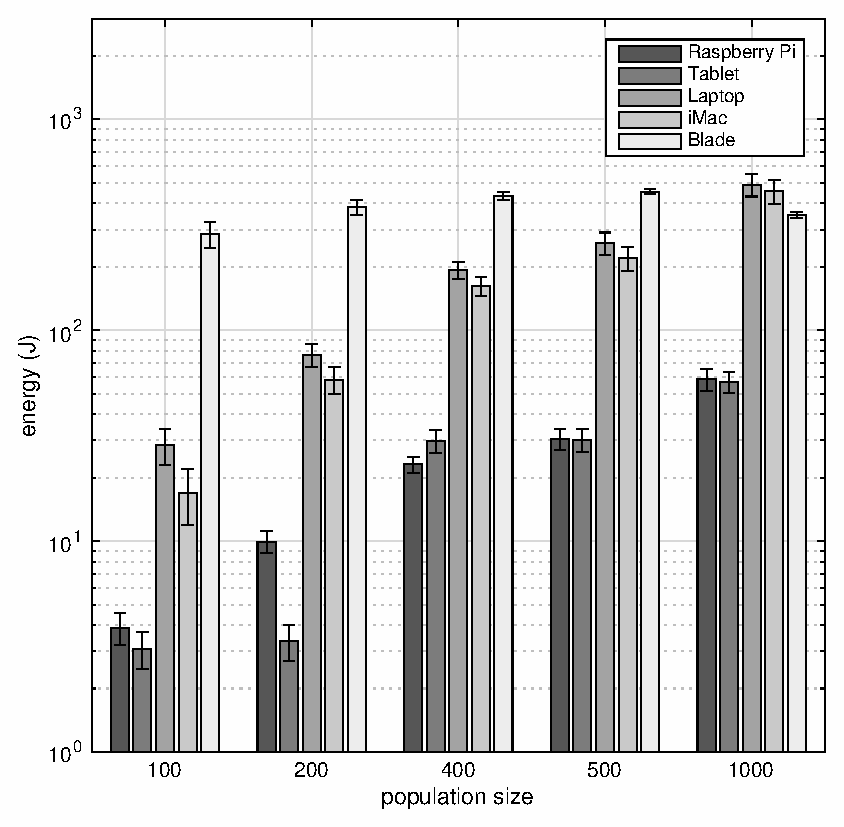
\includegraphics[width=.48\textwidth]{excess_energy_log_2.eps}}
\caption{(a) Instantaneous power delivered in each run. (b) Energy
  consumption per run. In both cases the bars (corresponding to
  \raspberrynsp, \tabletnsp, \laptopnsp, \iMac and \blade from left to
  right in each group) indicate mean values and the error bars span
  the standard error of the mean. Notice the logarithmic scale in the
  Y axis.\label{fig:powerenergy}} 
\end{figure}


\begin{figure}[!t]
\subfloat[\label{fig:fitness}]{\hspace{-1.2cm}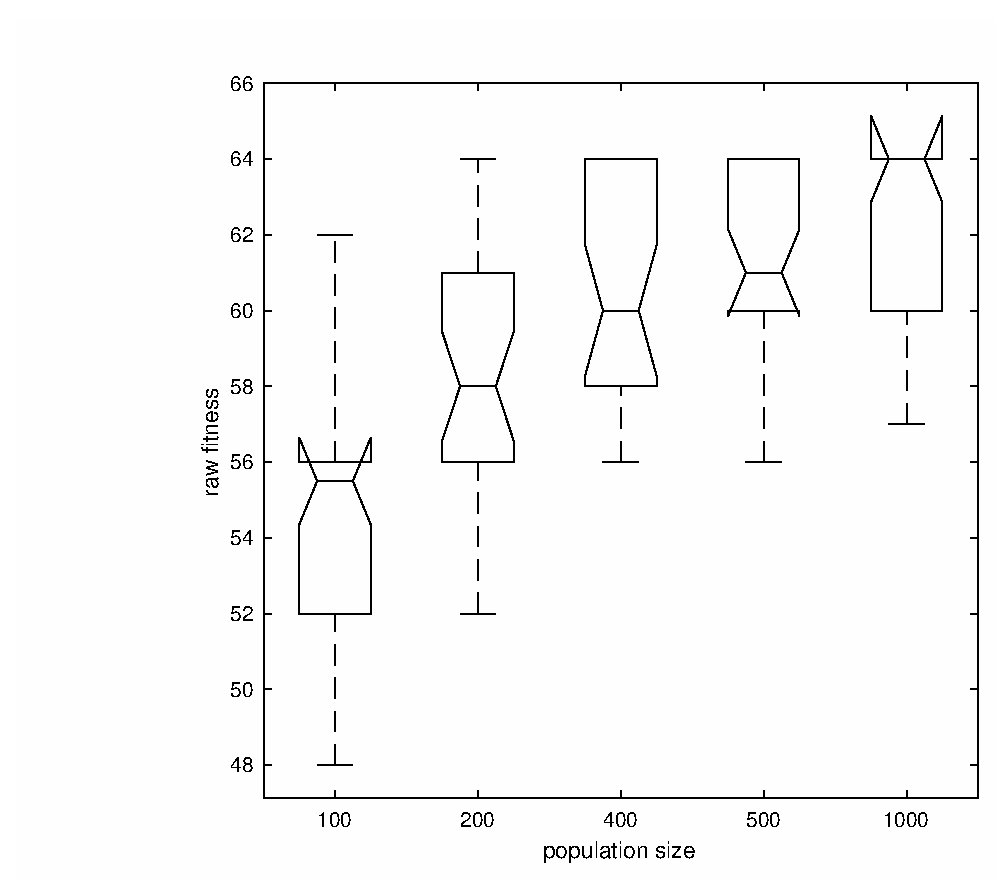
\includegraphics[width=.585\textwidth]{fitness.eps}}~~
\subfloat[\label{fig:powerlaw}]{\hspace{.2cm}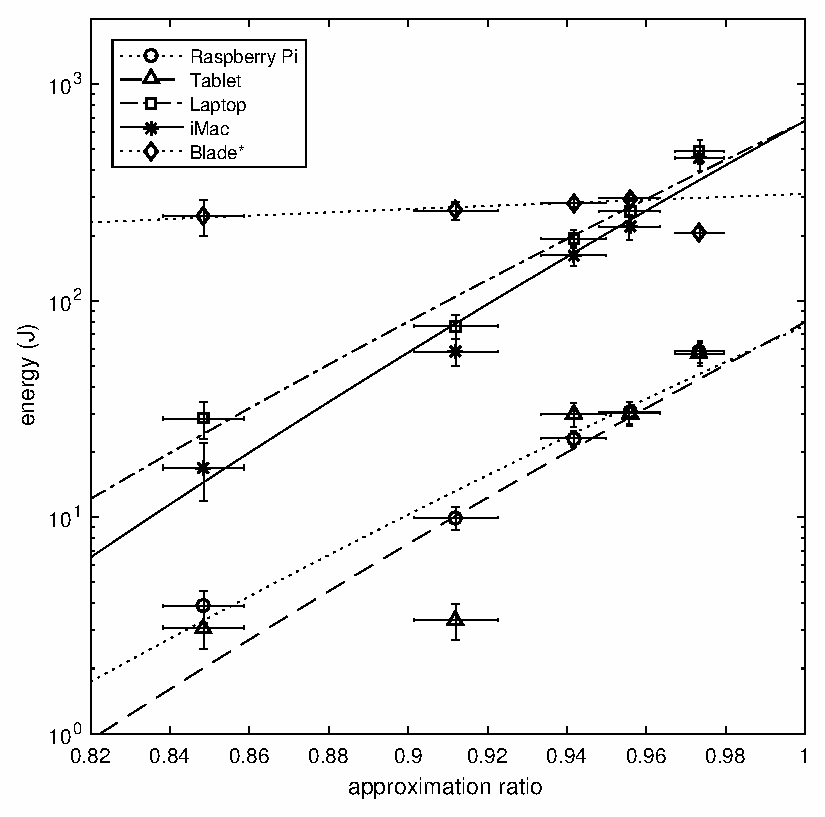
\includegraphics[width=.48\textwidth]{fitnessenergy.eps}}
\caption{(a) Distribution of fitness values attained for each population size (platform independent). 
(b) Trade-off between fitness attained and energy consumption. The
data points mark mean values and the error bars indicate the standard
error of the mean. A fit to a power-law $E\propto f^k$ is also
included (in the case of the \blade system, we have omitted the last
point since it is an outlier).%Maybe you should have omitted the fit - JJ
 Notice the logarithmic scale in the Y
axis. 
\label{fig:fitnessenergy}}
\end{figure}

As described in the previous section, computational times and power
delivered for each of the devices are reported in
Table~\ref{T:r_obtained}; algorithms tested using
different population sizes for each of the experiments are shown in
Fig.~\ref{fig:power}.  The
first thing that may be noticed is the difference in computing time
among devices analyzed, which corresponds with expectations:  small
devices (\raspberry and \tabletnsp) require quite a long time to reach
solutions and this is typically the reason why they are not frequently
used as the hardware platform to run EAs -- although they are useful
when non-standard distributed models are analyzed (such as pool-based
models, \cite{pool}). 

Nevertheless, we are considering a different point of view, and will
not just focus on computing time.  Different features can thus be
analyzed:  (i) device behavior when considering energy consumed by the
algorithm per unit of time; (ii) total energy required to find a
solution and (iii) the way population size influences the energy needs
when looking for a solution. If we focus firstly on the energy
required by {\tt lilgp} to be run in every device (see
Fig. \ref{fig:energy}), we notice that  handheld devices (\raspberry
and \tabletnsp) are the least demanding ones, requiring an order of
magnitude less energy to run the same algorithm when compared with
more standard computers:  \iMacnsp, \laptop and \blade
system. Secondly, when considering the total energy required to reach
the solution for the problem, the tablet running Android is the device
that provides the \emph{cheapest} solution, according to energy
consumed, while \blade and \laptop are the most \emph{expensive} ones
in every case.  Yet, if we only focus on computing time, the
opposite is the case, and \iMacnsp, \laptop and \blade would be the
preferred ones.  But given that we are looking for energy-efficient
ways of finding solutions by means of EAs, then \raspberry and \tablet
are preferred. 

Finally, we can also analyze %why? 
 the influence of population sizes in both
the time to reach solutions and the energy required for that.  In the
experimental stage, the runs with smaller population sizes typically
reach 500 generations -- the maximum allowed, given that they cannot
find the solution with that small number of individuals. % why did you
                                % use then? - JJ
 Therefore,
we will focus on the runs with larger population sizes and the energy
consumed to reach those solutions.  We see in Fig. \ref{fig:energy}
that there is a general trend of increasing energy cost for increasing
population sizes\footnote{@frchavez comment on blade} which has a
twofold cause: the longer computational time needed to complete the
runs and the slightly larger power delivered in each case. The latter
effect can be due to issues related to memory management % you should
                                % test this hypothesis, or say you
                                % will, in future work - JJ
and is most
remarkable in non-handheld devices (quite interestingly, no change is
found for \raspberry and quite small changes for the \tabletnsp). This
increased energy toll does not always pay off as we can see by
inspecting Fig. \ref{fig:fitness}; except for the largest population
size, there does not seem to be a significant difference between the
median fitness for a certain size and the immediately smaller size. A
more focused perspective on this issue is shown in
Fig. \ref{fig:powerlaw} in which we depict the energy required by each
device to attain a certain fitness. The order of growth of this cost
can be modeled as a power law as a first approximation. Such a power
law is consistent with the superlinear cost of obtaining increasingly
better approximations to the optimal solution and --while the fit can
be obviously improved-- it provides the means for a first comparison
of these different devices. Thus, we can see how the general trends
are not dramatically different for  \raspberrynsp, \tabletnsp, \laptop
and \iMac except for the offset of order of magnitude between the two
former and the two latter. The \blade system provides a more stable
energy profile and can be preferred to \laptop and \iMac if a tight
approximation to the optimum is sought. However, the smaller devices
remain the best option in terms of energy cost. 


%We may notice first large differences in energy required to run the GP algorithm, when different hardware devices are employed.  Thus, raspberry pi and tablet devices are the ones requiring smaller amounts of energy per unit of time (power).  Nevertheless, when we take into account not only power, but also total time to complete an experiment, and given that laptops and blade systems provide better computing capabilities, things could be different.  N


 %(~\ref{fig:consumo}). 

%\begin{figure}[ht]%
	%\centering
 	%\includegraphics[width=0.3\textwidth]{./Resultados/consumos.pdf}
 	%\caption{Consumo (w) del SoC en la implementación final del algoritmo.}
  %\label{fig:consumo} 
%\end{figure}



%\begin{figure}[ht]%
	%\centering
 	%\includegraphics[width=0.3\textwidth]{./Resultados/voltimetro.pdf}
 	%\caption{Voltímetro utilizado para la toma de medidas de potencia en los resultados experimentales.}
  %\label{fi:voltimetro} 
%\end{figure}


%Table~\ref{Table:result_todos} shows results obtained with a population size of 100, 200, 400, 500 and y 1000 individuals, respectively. 

%\begin{small}
%
%\begin{table}[!ht]
%\renewcommand{\arraystretch}{1.3}
%\centering
%\caption{Experimental results - GP - Multiplexer 6}
%\label{Table:result_todos}
%\begin{tabular}{ccccc} \hline
%Device & Power (W) & Time (sec.) & Energy (Joules) & (Kwh) \\ \hline
%\multicolumn{4}{c}{\textbf{Population size = 100}}\\ %\hline
%Raspberry Pi & 0.5 & 233.14 &116.57 & $3.24*10^{-5}$ \\
%Tablet & 0.63 & 132.75 & 83,3 & $2.31*10^{-5}$ \\
%Mac & 12.26 & 41.51 & 508,91 & $1.41*10^{-4}$ \\
%Laptop & 16.49 & 51.79 & 853.95 & $2.37*10^{-4}$ \\
%Blade & 13.8 & 77.84 & 1074.19 & $2.98*10^{-4}$ \\ \hline
%\multicolumn{4}{c}{\textbf{Population size = 200}}\\ %\hline
%Raspberry Pi & 0.5 & 597.29 & 298.64 & $8.30*{-5}$ \\
%Tablet & 0.63 & 145.63 & 92.9 & $2.56*10^{-5}$ \\
%Mac & 14.87 & 110.58 & 1644.32 & $3.77*10^{-4}$ \\
%Laptop	& 17.38 & 132.88 & 2309.41 & $6.42*10^{-4}$ \\
%Blade & 18.71 & 206.48 & 3863.24 & $1.07*10^{-3}$ \\ \hline
%\multicolumn{4}{c}{\textbf{Population size = 400}}\\ %\hline
% Raspberry Pi & 0.5 & 1386.52 & 693.26 & $1.93*10^{-4}$ \\
%Tablet & 0.82 & 1070.26 & 873.1 & $2.43*10^{-4}$\\
%Mac&17.49 & 269.38 & 4711.68 & $1.11*10^{-3}$\\
%Laptop & 18.25 & 317.98 & 5803.17 & $1.61*10^{-3}$\\
%Blade & 21.17 & 503.33 & 10655.5 & $2.96*10^{-3}$ \\ \hline
%\multicolumn{4}{c}{\textbf{Population size = 500}}\\ %\hline
%Raspberry Pi & 0.5 & 1833.07 & 916.53 & $2.55*10^{-4}$ \\
%Tablet & 0.82 & 1085.17 & 890.56 & $2.47*10^{-4}$ \\
%Mac & 18.75 & 352.31 & 6605.81 & $1.83*10^{-3}$ \\
%Laptop & 18.58 & 416.76 & 7743.73 & $2.15*10^{-3}$ \\
%Blade & 22.19 & 668.54 & 14834.90 & $4.12*10^{-3}$ \\ \hline
%\multicolumn{4}{c}{\textbf{Population size = 1000}}\\ %\hline
%Raspberry Pi & 0.5 & 3504.14 & 1752.07 & $4.87*10^{-4}$ \\
%Tablet & 0.82 & 2060.85 & 1686.49 & $4.68*10^{-4}$ \\
%Mac & 19.89 & 688.63 & 13696.85 & $3.80*10^{-3}$ \\
%Laptop & 19.01 & 813.78 & 15469.93 & $4.30*10^{-3}$ \\
%Blade &	17.1 & 1305.84 & 22329.86 & $6.20*10^{-3}$ \\ \hline
%
%\end{tabular}
%\end{table} 
%\end{small}


%Table~\ref{Table:result_ga} shows GA results when using population sizes: 50, 100, 500 y 1000.

%\vspace{-0.5cm}
%\begin{table}[!ht]
%\renewcommand{\arraystretch}{1.3}
%\centering
%%\tiny
%\caption{Experimental Results - GA}
%\label{Table:result_ga}
%\begin{tabular}{cccc} \hline
%Device & Power (W) & Time (seg.) & Energy (Kwh) \\ \hline
%\multicolumn{4}{c}{\textbf{Population size = 50}}\\ %\hline
% Raspberry Pi & 0,32 & 41,66 &  $0,370*10^{-5}$ \\
% Laptop & 12,76 & 5,1 & $1,81*10^{-5}$ \\
% Smartphone & 0,27 & 35,48 & $0,272*10^{-5}$ \\
% FPGA & 1,982 & 60,523 & $3,332*10^{-5}$\\  \hline
%\multicolumn{4}{c}{\textbf{Population size = 100}}\\ %\hline
% Raspberry Pi & 0,32 & 109,89 &  $0,977*10^{-5}$ \\
% Laptop & 15,76 & 12,11 & $5,3*10^{-5}$ \\
% Smartphone & 0,26 & 65,75 & $0,48*10^{-5}$ \\
% FPGA & 1,990 & 153,06 & $8,4608*10^{-5}$ \\ \hline
%\multicolumn{4}{c}{\textbf{Population size = 500}}\\ %\hline
% Raspberry Pi & 0,38 & 996,61 &  $10,520*10^{-5}$ \\
% Laptop & 18,6 & 87,16 & $45,034*10^{-5}$ \\
% Smartphone & 0,18 & 802,26 & $4,185*10^{-5}$ \\
% FPGA & 2,050 & 964,27& $54,909*10^{-5}$\\ \hline
%\multicolumn{4}{c}{\textbf{Population size = 1000}}\\ %\hline
% Raspberry Pi & 0,5 & 2572,8 &  $35,733*10^{-5}$ \\
% Laptop & 19,49 & 215,33 & $116,475*10^{-5}$ \\
% Smartphone & 0,22 & 2219,80 & $13,807*10^{-5}$ \\
% FPGA & 2,172 &2429,97 & $146,60*10^{-5}$\\ \hline
%\end{tabular}
%\end{table} 
%%\vspace{-0.5cm}




\section{Conclusions}
\label{conclusions}

We have presented a preliminary study on the energy consumed by a well
known EA: the Genetic Programming algorithm. We 
have analyzed the behavior of a benchmark GP problem, the
multiplexer-6, and have run it using {\tt lilgp} on different
hardware devices running a number of operating systems, from blade
systems using different Linux distributions to tablet devices running
Android. 

One of the first things we have learned is that although devices with
better processors can run the algorithm faster, they spend
larger amounts of energy, and the total energy required to find a
solution is also larger.  This means that although the standard
preference for better hardware platforms and processors allows to find
solutions more quickly, it incurs in waste of energy that should be
considered:  it is much more energy efficient to run the algorithm on
a Raspberry Pi or a tablet device. Of course, it is expected that some very 
computationally-expensive problems could not be fully solved in one
of these devices. Then again, they can provide a valuable, energy-efficient
contribution to the collective resolution of such problems when used
within a larger ephemeral network of computing devices \cite{ephemeral2015}.

Secondly, we have seen the influence of one of the main parameters
of the algorithm may have on the energy consumed:  changing population
sizes automatically produce a change in the amount of energy required to reach
solutions, and this is a hint on future analysis.  We should thus carefully
consider how each of the parameters of the algorithm may also
influence the amount of energy consumed when looking for solutions. 

As a future line of work, it would be interesting to consider
different devices in the same class exploring the space of
solutions in a multiobjective way: which devices manage to find the
solution faster for the least amount of energy?  In principle the analysis
is generic and does not rely on any 
feature that could be said to be GP-specific, so we believe the conclusions
extracted are applicable to any EA.  This said, it would be also interesting to further confirm
this. We will thus expand the study
to other evolutionary algorithms to check whether these energy
profiles are exclusive of GP or there are variations
among them. Energy profiling the algorithms will also allow us to find
out where the energy expenses actually come from, allowing us to
optimize the algorithm itself making it energy-aware.

\subsubsection*{Acknowledgements}
\sloppypar We acknowledge support from 
Spanish Ministry of Economy and Competitiveness and European Regional
Development Fund (FEDER) under project EphemeCH
(TIN2014-56494-C4-\{1,2,3\}-P),  
from University of Granada, PROY-PP2015-06 (Plan Propio 2015 UGR), 
from Junta de Andaluc\'{\i}a under project DNEMESIS (P10-TIC-6083),
from Universidad de M\'alaga, Campus de Excelencia Internacional
Andaluc\'{\i}a Tech,  
from Junta de Extremadura FEDER, project GR15068 and FP7-PEOPLE-2013 IRSES Grant 612689 ACoBSEC.

%----------------------------------------------------------------------------------------
%	REFERENCE LIST
%----------------------------------------------------------------------------------------
 
\begin{thebibliography}{99} % Bibliography - this is intentionally simple in this template

\bibitem{smith}{Smith, S. F. (1980). \textit{A Learning System Based on Genetic Adaptive Algorithms}. PhD thesis, Computer Science Department, University of Pittsburgh.}
\bibitem{soule}{Soule, T. and Foster, J. A. (1998a). Effects of code growth and parsimony pressure on populations in genetic programming. \textit{Evolutionary Computation}, 6(4):293-309.}
\bibitem{tackett}{Tackett, W. A. (1994). \textit{Recombination, Selection, and the Genetic Construction of Computer Programs}. PhD thesis, University of Southern California, Department of Electrical Engineering Systems.}
\bibitem{kalganova}{Kalganova, T. and Miller, J. (1999). Evolving more efficient digital circuits by allowing circuit layout evolution and multi-objective fitness. In Stoica, A., Keymeulen, D., and Lohn, J., editors, \textit{Proceedings of the 1st NASA/DoD Workshop on Evolvable Hardware (EH’99)}, pages 54-63, Piscataway, NJ. IEEE.}
\bibitem{zhang}{Zhang, B.-T. and Muhlenbein, H. (1995). Balancing accuracy and parsimony in genetic programming. \textit{Evolutionary Computation}, 3(1):17-38.}
\bibitem{nedja}{Nedja, N., Abraham, A., and de Macedo Mourelle, L. editors (2006). \textit{Genetic Systems Programming}. Springer.}
\bibitem{silva}{Silva, S. and Almeida, J. (2003). Dynamic maximum tree depth. In \textit{Genetic and Evolutionary Computation, GECCO-2003}, pages 1776-1787, Chicago. Springer.}
\bibitem{green-computing}{Hooper, A. (2008). Green computing. Communication of the ACM, 51(10), 11-13.}
\bibitem{HVAC}{Fong, K. F., Hanby, V. I., Chow, T. T. (2006). HVAC system optimization for energy management by evolutionary programming. Energy and Buildings, 38(3), 220-231.}
\bibitem{chiller}{Lee, W. S., Chen, Y. T., Kao, Y. (2011). Optimal chiller loading by differential evolution algorithm for reducing energy consumption. Energy and Buildings, 43(2), 599-604.}
\bibitem{dispatch}{Fadaee, M., Radzi, M. A. M. (2012). Multi-objective optimization of a stand-alone hybrid renewable energy system by using evolutionary algorithms: A review. Renewable and Sustainable Energy Reviews, 16(5), 3364-3369.}
\bibitem{self}{Cotta, C. Fernández, A. J., Fernández de Vega, F., Chávez, F., Merelo, J.J.,Castillo, P.A., Camacho, D., Bello, G:
Ephemeral Computing and Bioinspired Optimization. IJCCI (ECTA) 2015: 319-324}
\bibitem{energy-aware}{Yoo, C. M. K. S. (2011). Energy-Aware System Design.}
\bibitem{cache}{Díaz, J., Risco, J.L., Colmenar, J.M., Multi-objective optimization of energy consumption and execution time in a single level cache memory for embedded systems.}
\bibitem{scaling}{Bansal, N., Kimbrel, T., Pruhs, K. (2004, October). Dynamic speed scaling to manage energy and temperature. In Foundations of Computer Science, 2004. Proceedings. 45th Annual IEEE Symposium on (pp. 520-529). IEEE.}
\bibitem{dynamic-scaling}{Albers, S. (2011). Algorithms for dynamic speed scaling. In LIPIcs-Leibniz International Proceedings in Informatics (Vol. 9). Schloss Dagstuhl-Leibniz-Zentrum fuer Informatik.}
\bibitem{energy-efficient}{Albers, S. (2010). Energy-efficient algorithms. Communications of the ACM, 53(5), 86-96.}
\bibitem{michalewicz}{Zbigniew Michalewicz,(1996). Genetic Algorithms + Data Structures = Evolution Programs. Third Edition, Springer.  ISBN: 3-540-60676-9.}
\bibitem{cantupaz}{Cantu-Paz, E. (2000). Efficient and Accurate Parallel Genetic Algorithms, ser. Book Series on Genetic Algorithms and Evolutionary Computation.}
\bibitem{fcofdez}{Fernández, F., Tomassini, M., Vanneschi, L. (2003). An empirical study of multipopulation genetic programming. Genetic Programming and Evolvable Machines, 4(1), 21-51.}
\bibitem{web_algoritmo}{Dennis Cormier and Sita Raghavan. http://people.sc.fsu.edu/~jburkardt/cpp\_src/ simple\_ga/simple\_ga.html.}
\bibitem{complexity}{Papadimitriou, C. H. (2003). Computational complexity (pp. 260-265). John Wiley and Sons Ltd..}
\bibitem{ephemeral}{Cotta, C., Fernández, A., Fernández de Vega, F, Chávez, F., Merelo, J.J., Castillo, P., Camacho, D., Bello, G., Ephemeral computing and bioinspired optimization:  challenges and opportunities.  Proceedings ECTA 2015.}
\bibitem{paba}{Fernández de Vega, F., Pérez, J. I. H. (2012). Parallel Architectures and Bioinspired Algorithms (Vol. 122). Springer.}
\bibitem{powertutor}{Gordon, M., Zhang, L., Tiwana, B., Dick, R., Mao, Z. M., Yang, L. (2013). PowerTutor: a power monitor for android-based mobile platforms.}
\bibitem{powertutor2}{Zhang, L., Tiwana, B., Qian, Z., Wang, Z., Dick, R. P., Mao, Z. M., Yang, L. (2010, October). Accurate online power estimation and automatic battery behavior based power model generation for smartphones. In Proceedings of the eighth IEEE/ACM/IFIP international conference on Hardware/software codesign and system synthesis (pp. 105-114). ACM.}
\bibitem{lilgp}{Punch, B., Zongker, D. (1998). Lil-gp genetic programming system. Software from site Michigan State University GARAGe.}
\bibitem{barroso2007case}{Barroso, L.A. and H{\"o}lzle, U. (2007). The case for energy-proportional computing. Computer, Vol. 12, pp. 33-37. IEEE}
\end{thebibliography}


%----------------------------------------------------------------------------------------

\end{document}
